\documentclass{article}

\usepackage[utf8]{inputenc}
\usepackage{amsmath}
\usepackage{amssymb}
\usepackage{anysize}
\usepackage{color}
\usepackage{xcolor}
\usepackage{graphicx}
\usepackage{float}


\newcommand{\BigO}[1]{\ensuremath{\operatorname{O}\bigl(#1\bigr)}}

\usepackage{listings}
\lstset{
	language=C++,                	% choose the language of the code
	basicstyle=\footnotesize,       % the size of the fonts that are used for the code
	numbers= left,                 	% where to put the line-numbers
	numberstyle=\footnotesize,      % the size of the fonts that are used for the line-numbers
	stepnumber=1,                   % the step between two line-numbers. If it is 1 each line will be numbered
	numbersep=5pt,                  % how far the line-numbers are from the code
	backgroundcolor=\color{white},  % choose the background color. You must add \usepackage{color}
	showspaces=false,               % show spaces adding particular underscores
	showstringspaces=false,         % underline spaces within strings
	showtabs=false,                 % show tabs within strings adding particular underscores
	frame=single,           		% adds a frame around the code
	tabsize=2,          			% sets default tabsize to 2 spaces
	captionpos=t,          			% sets the caption-position to bottom (t=top, b=bottom)
	breaklines=true,        		% sets automatic line breaking
	breakatwhitespace=false,    	% sets if automatic breaks should only happen at whitespace
	escapeinside={\%*}{*)}          % if you want to add a comment within your code
}



\usepackage{caption}
\DeclareCaptionFont{white}{\color{white}}
\DeclareCaptionFormat{listing}{\colorbox{gray}{\parbox[c]{\textwidth}{#1#2#3}}}
\captionsetup[lstlisting]{format=listing,labelfont=white,textfont=white}

\setlength\parindent{0pt}
\setlength{\parskip}{10pt}

\marginsize{3cm}{2cm}{2cm}{2cm}

\title{Sensors and Digitization\\
		Moving Object Imaging\\
		Lab 5 Report\\
		GrTP1A}
\author{Daniel Sileshi Asfaw\\
		Emre Ozan Alkan\\}
\date{26 November 2013}

\begin{document}
\maketitle

\section{Objective}
	In this lab, our objective was to study imaging solutions to analyze moving objects with line-scan camera systems and understand their specific features. Specifically,
	\begin{itemize}
		\item Capture images of moving object at different speed
		\item Study the parameters affecting moving object imaging techniques
		\item Properly calibrate our camera to get real image of the moving object
		\item Change the exposure time of line scanning camera using external triggering.
	\end{itemize}

	\subsection{Equipment}
	In the lab room, we had following equipment to use:
	\begin{itemize}
		\item PC Computer
		\item Frame Grabber: DALSA XCELERA-CL LX1
		\item Digital Camera: DALSA S2-1X-02K40
		\item 50 nm Lens: PENTAX YF5028A-02
		\item Video Cables
		\item 12V Power Supply
		\item Moving Industrial Parts
		\item Signal Generator
		\item Oscilloscope
	\end{itemize}		
	
	\subsection{Software}
	We used the following software in the lab computers:
	\begin{itemize}
		\item CamExpert - TELEDYNE DALSA
	\end{itemize}
	
	\subsection{Documentation}
	Here is the documentations we followed during the lab session;
	\begin{itemize}
		\item User Manual \& Brochure for camera \& frame grabber
		\item Lectures notes on Machine Vision
	\end{itemize}
	
	
\section{Preliminary}
	This laboratory session had two experiments. The first experiment was grabbing image of a moving object without using any external triggering system and the second was using external triggering to grab image of and object at different triggering frequencies.
	\begin{center}
	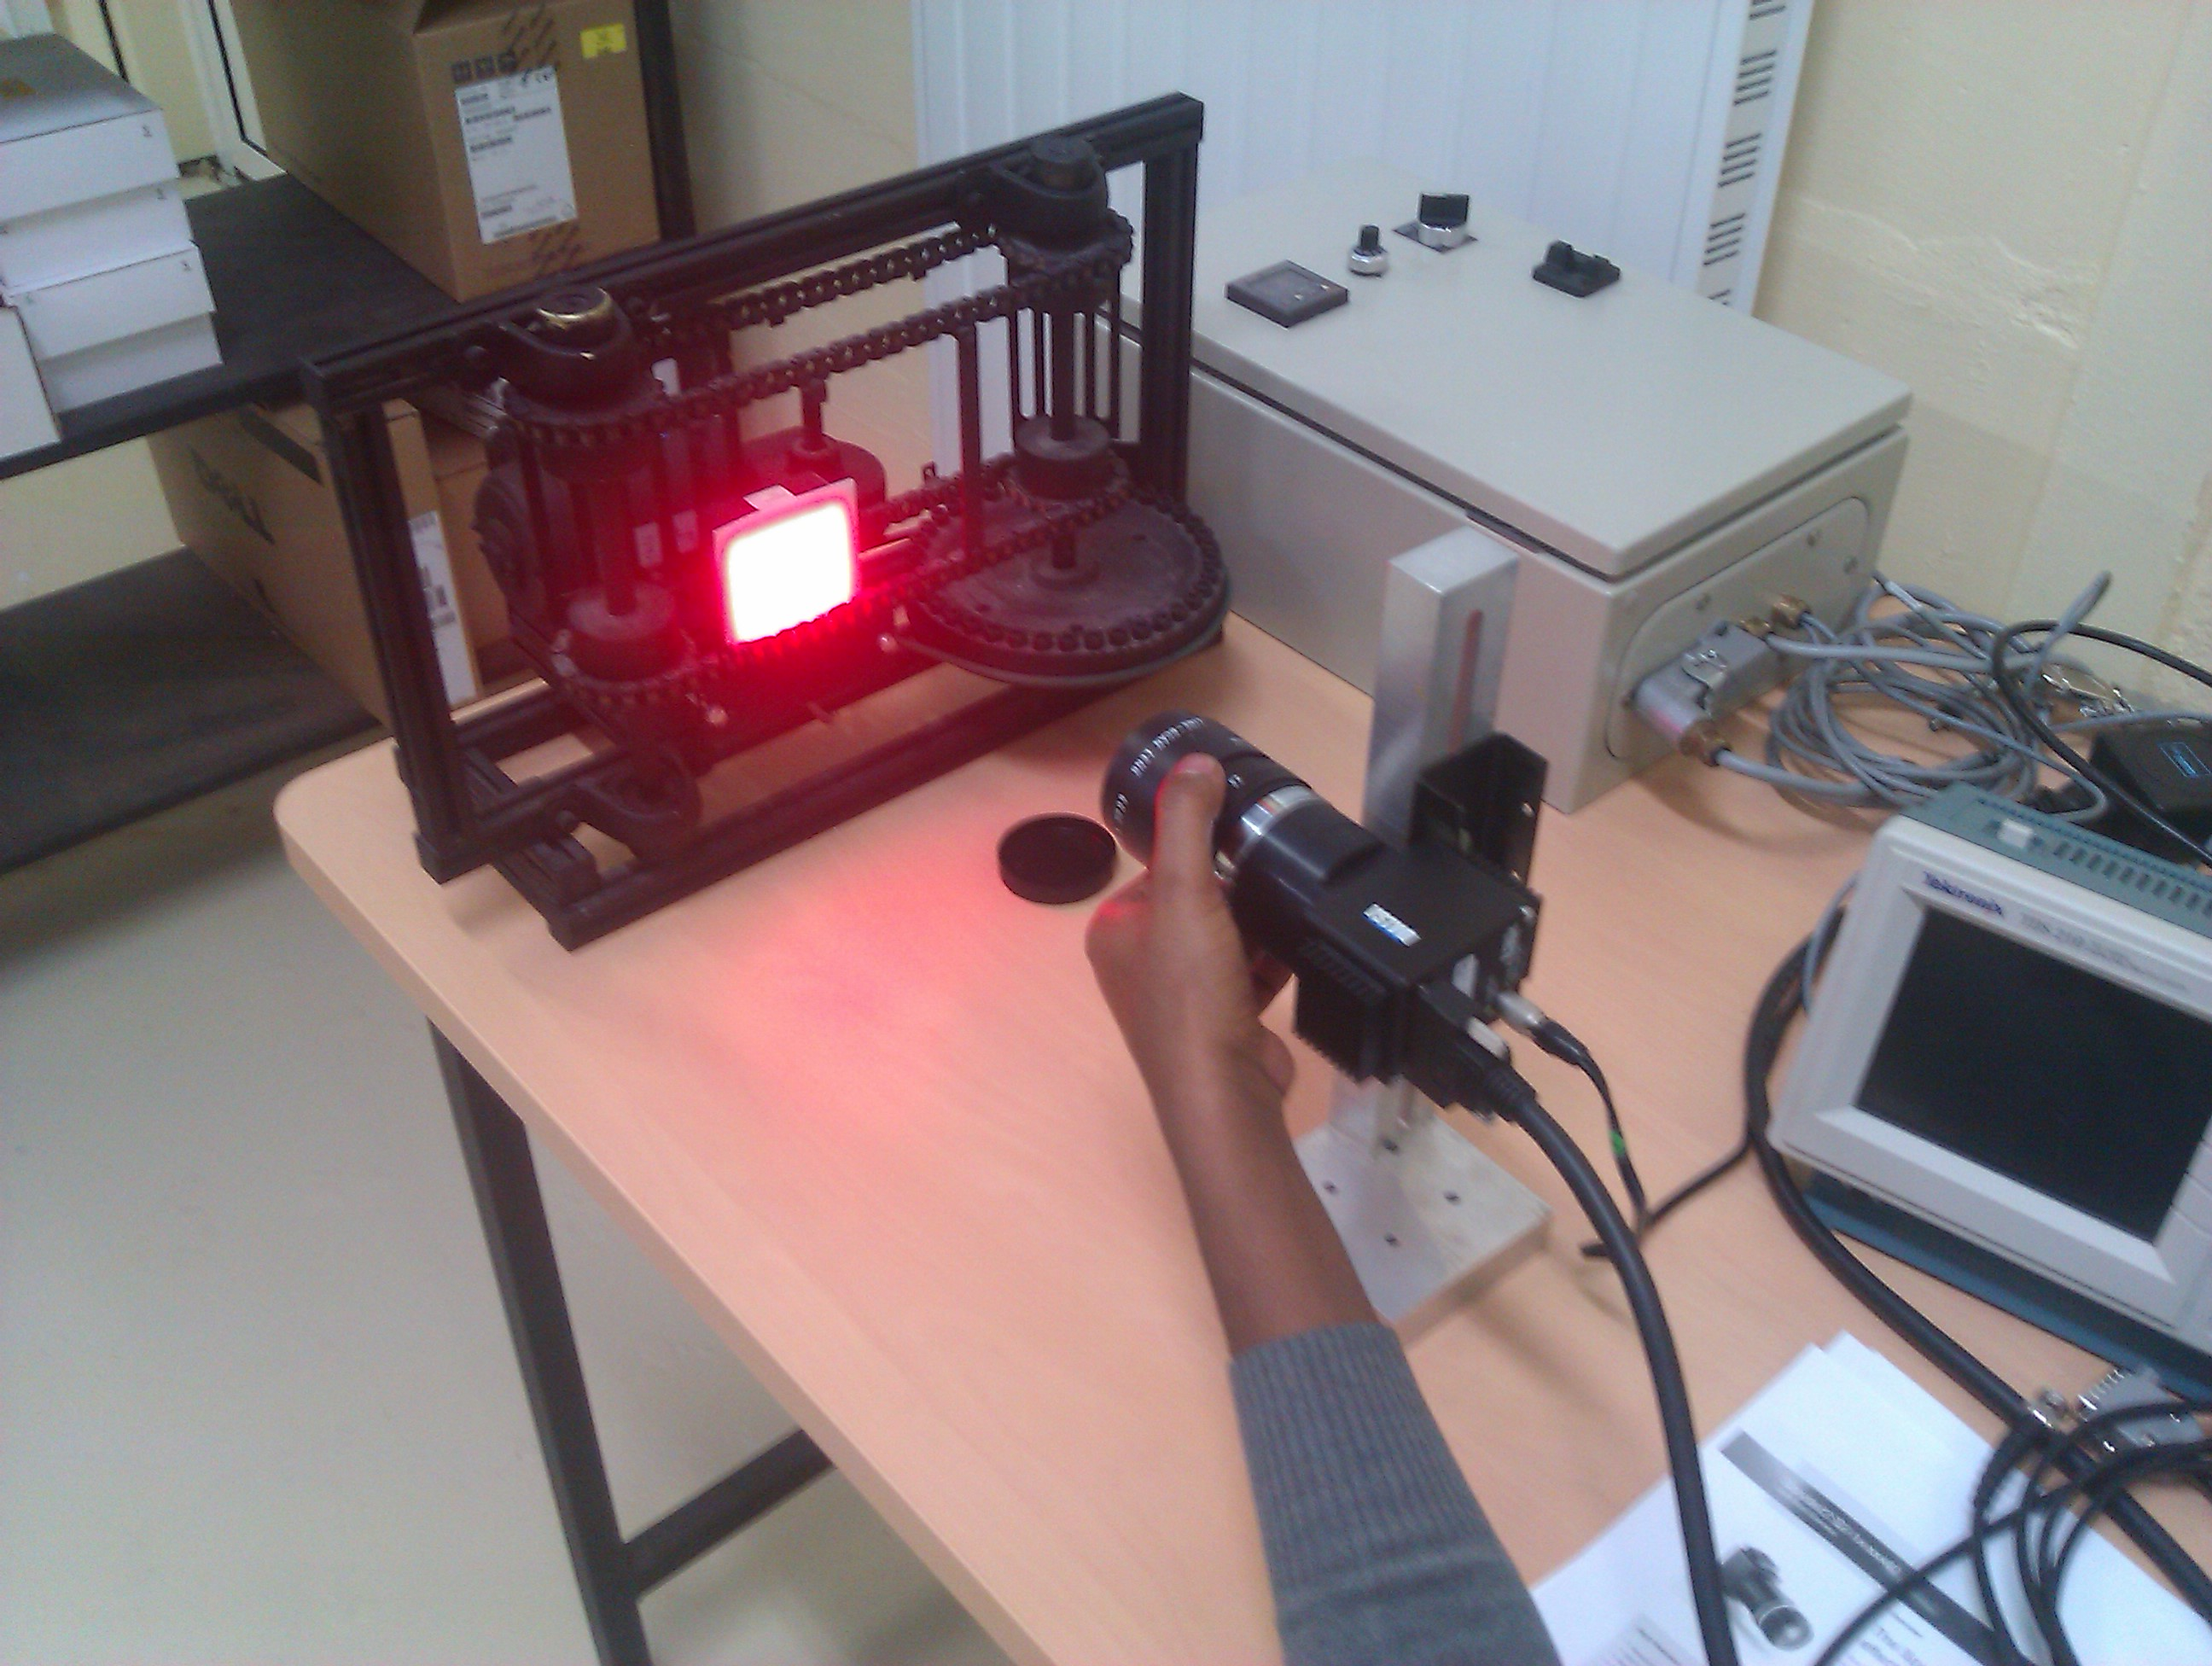
\includegraphics[scale=0.1]{setupPhoto.jpg}
	\end{center}
	\subsection{Experiment 1}
	In part of the lab session, we studied how to capture image of a moving object without using external triggers. Line camera is connected to the computer. Then, we have switched on the back-light of the image plane and moving industrial part motor. After we have launched the "Cam Expert" software on the computer to grab and image. We used the default line scanning parameters of the software.
	We also had adjusted the position of the camera, aperture and focus settings of the camera to capture a good image.
	\begin{center}
	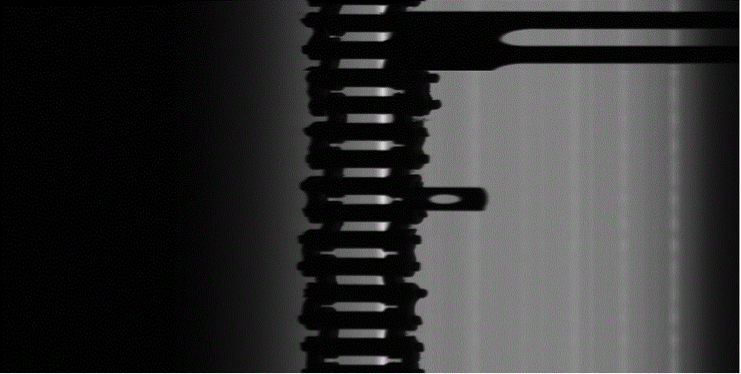
\includegraphics[scale=1.0]{objectPhoto.png}
	\end{center}
	\subsubsection{Observations}
	After setup everything, we started to take pictures via software. Our observation on taken pictures shows that, changing speed of the moving objects affects on its size. In faster speeds, object was more likely to appear more narrow and small. However, even we decrease the speed, object didn't appeared in its original ratio, but just slightly better than faster moving. The camera we were using was a line scanner type with resolution up to 512 to 2048, 18 to 65kHz line/frame rate, which is high dynamic range. The lines that camera scans, even scene is moving, is mostly the under-sampled samples and not representing the moving scene in actual size. So we end up needing external trigger to sync moving object and the capture of the line scanner with external frequency.
	
	\subsection{Experiment 2}
	In the second part of the experiment, we used an external trigger to grab an image. In order to do this, the triggering frequency from the signal generator is adjusted by connecting it with oscilloscope. Then, we connected the output of the signal generator to the computer. Since we were using the internal triggering mode for "Experiment 1", we changed the configuration on software to use external triggering mode. So we wanted to solve under-sampling issue with setting rate of line scan to avoid effects of the speed of moving object.
	
	\begin{center}
	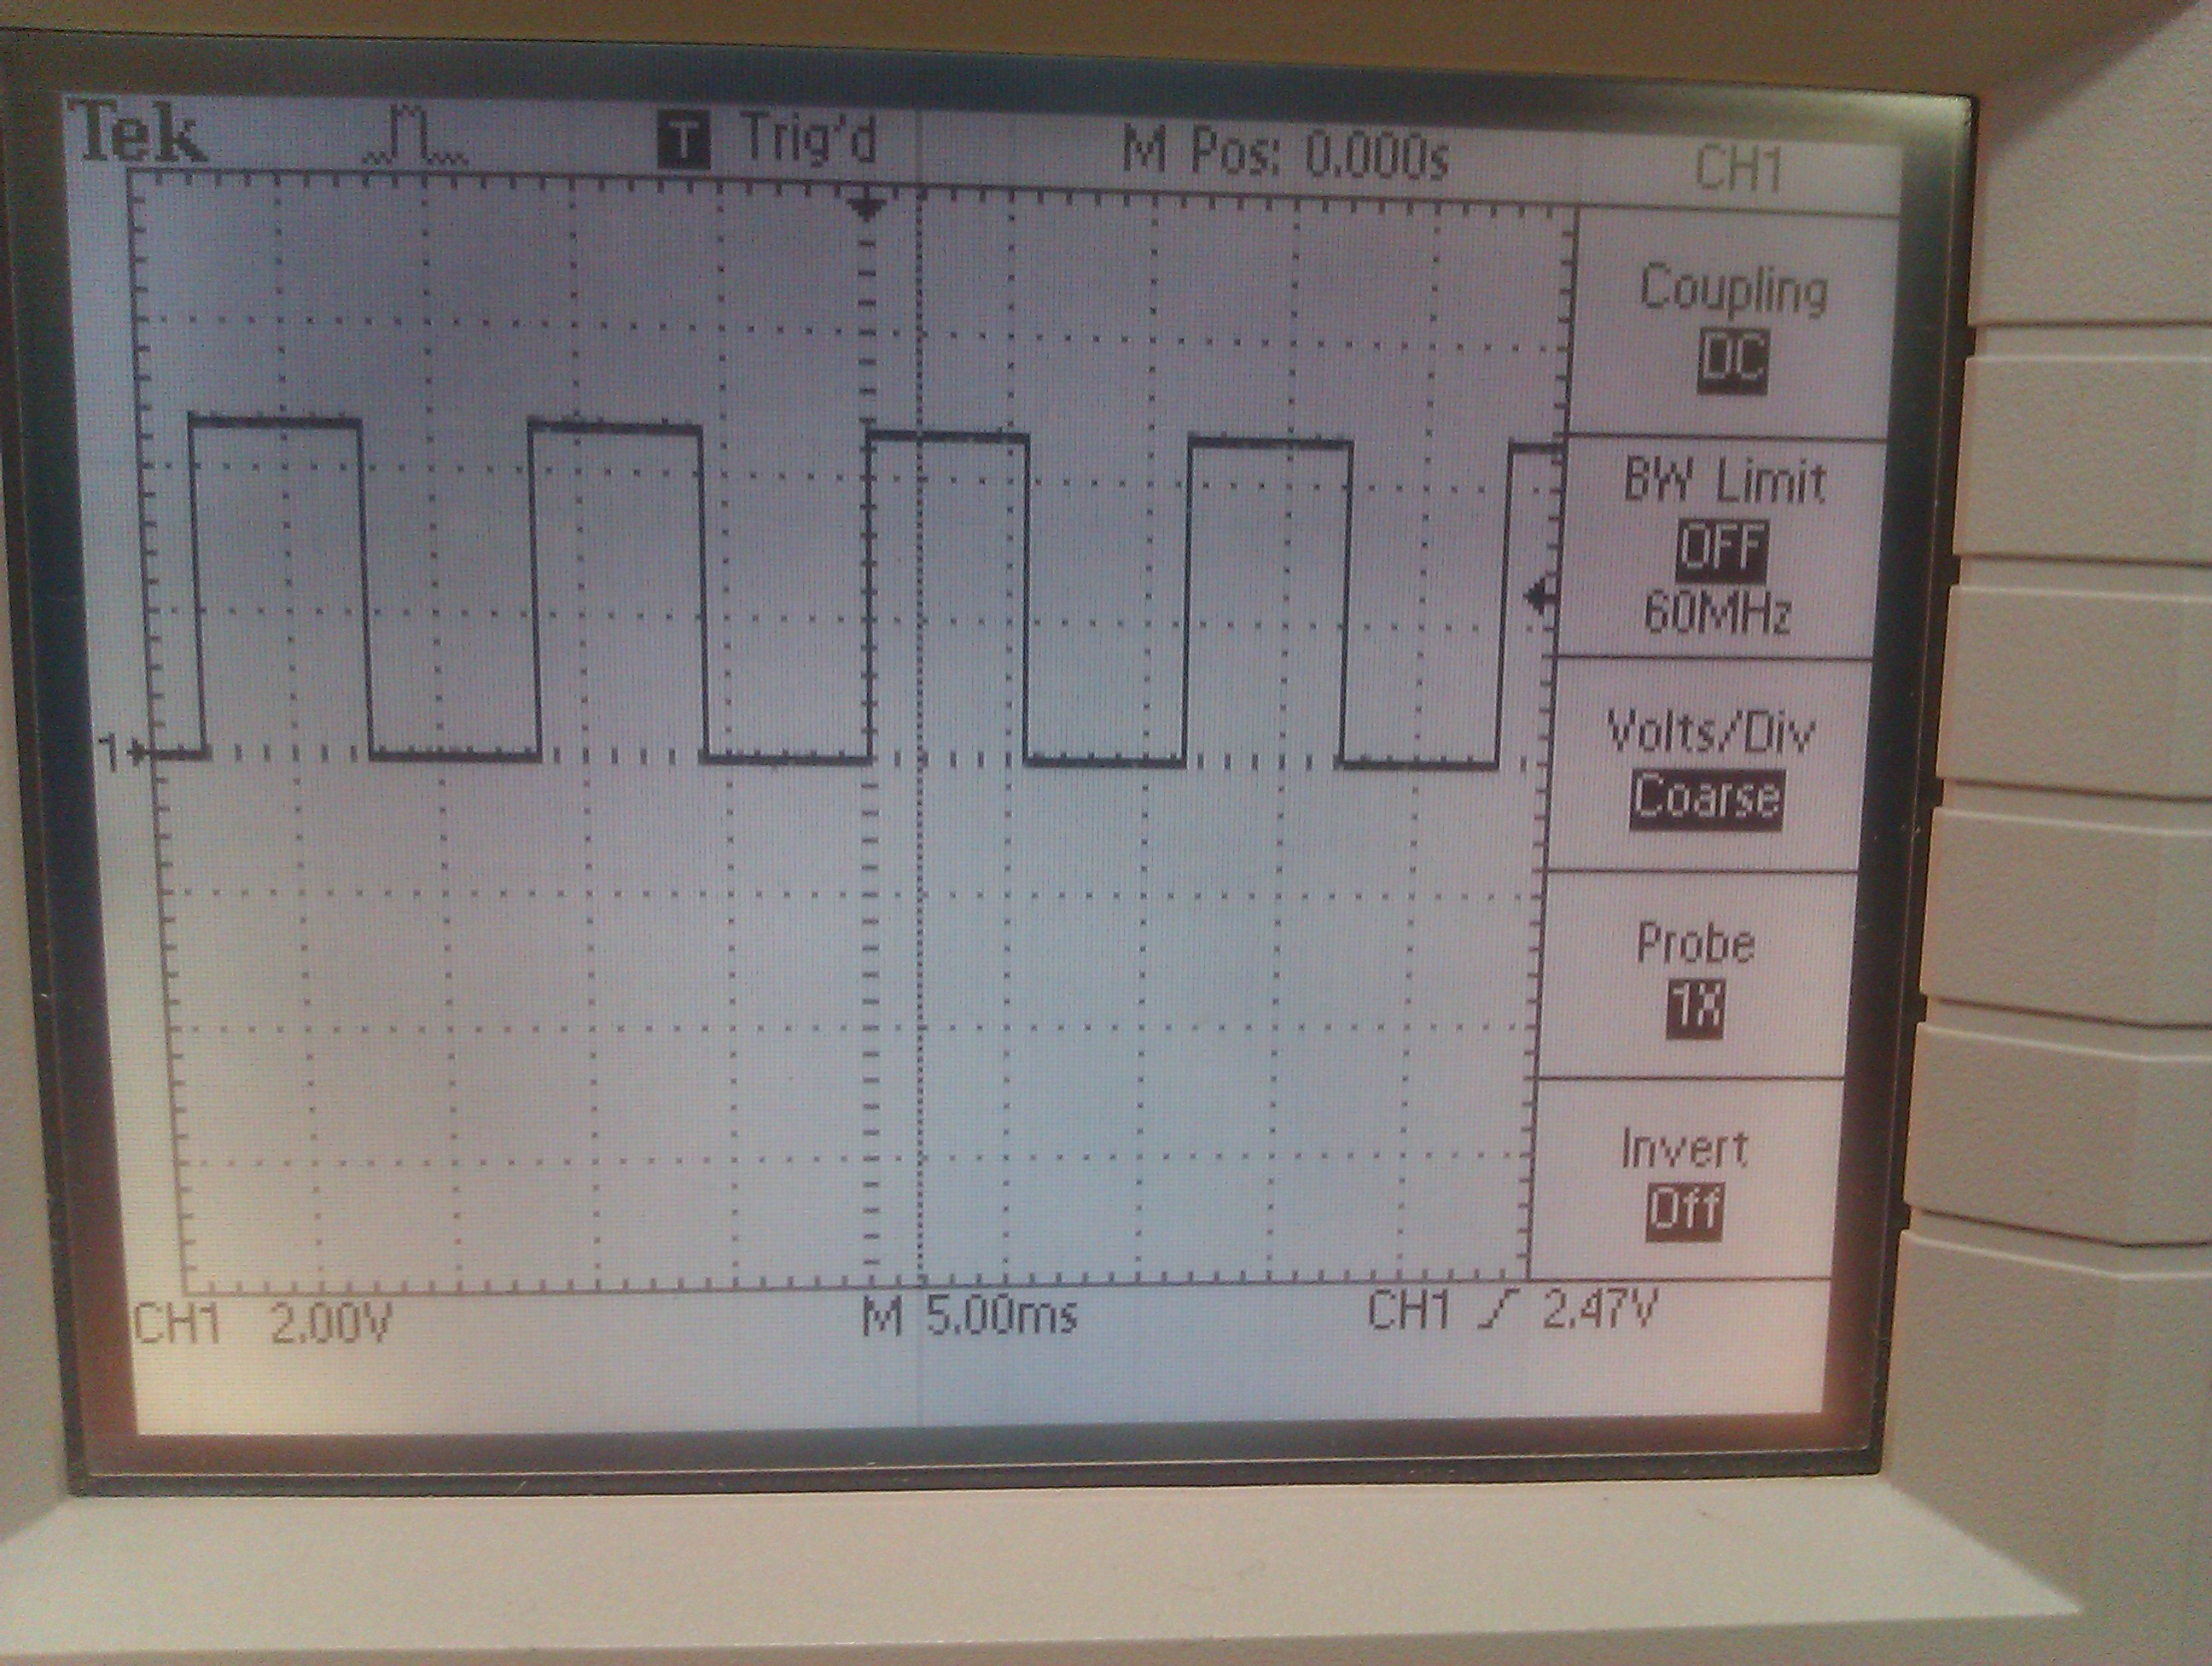
\includegraphics[scale=0.09]{signalPhoto.jpg}
	\end{center}
	
	\subsubsection{Observations}
	In the second experiment we seen that we can increase the frame rate of the camera via external triggering so that line scanner can get enough time and example to work with. Also decreasing the duty time, we achieved this by decreasing the pulse duration of our rectangular wave, which is responsible for exposure time, we had able to see more details on our object like text on it.
	
	
	
\section{Conclusion}
	Another lab with lessons, showed us that moving object imaging is not easy, and there is lots of parameters to know and setup. Also showed us a good application of line scanner cameras, not to go always with matrix cameras to study imaging. In conclusion, this lab gave us good concept of imaging moving objects with line scanner camera, and study the settings which affecting sensitively on the quality of images we can capture.
	
	

\end{document}
